\begin{frame}{PHP}
    \begin{figure}
        \centering
        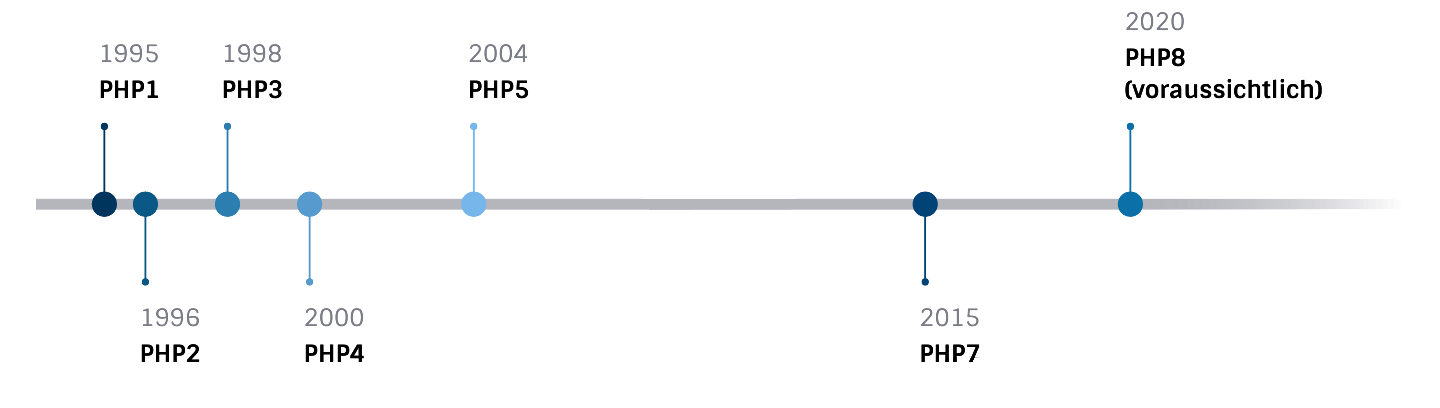
\includegraphics[width=290px]{img/timeline.png}	
        \caption{Major-Releases von PHP im Zeitverlauf}		
    \end{figure}
\end{frame}

\begin{frame}{Versionierung von Software}
    Semantic Versioning \nocite{preston-werner_semantic_nodate}:
    \begin{center}
        \alert{Major.Minor.Patch[-Pre-Release]}
    \end{center}
    \begin{itemize}
        \item \textbf{Major}: inkompatible API-Änderungen
        \item \textbf{Minor}: abwärtskompatible Änderungen oder \emph{Deprecations}
        \item \textbf{Patch}: abwärtskompatible Bugfixes
    \end{itemize}
\end{frame}

\begin{frame}{Versionierung von Software}
    \begin{figure}
        \centering
        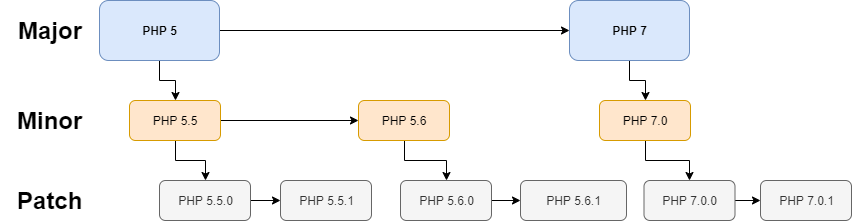
\includegraphics[width=270px]{img/semVer.png}
        \caption{Semantic Versioning am Besipiel von PHP}			
    \end{figure}
\end{frame}

\begin{frame}{ISO/IEC 14764}
    ,,Fahrplan'' zur Migration \nocite{iso/iec_iso/iec/ieee_2006}:
    \begin{itemize}
        \item Anforderungsanalyse und Definition der Migration
        \item Entwicklung von Werkzeugen zur Migration
        \item Entwicklung der angepassten Software
        \item Verifikation der Migration
        \item Support der alten Umgebung
    \end{itemize}
\end{frame}

